% ============================================================================
%  Group 22 - Machine Learning, NOVA IMS
%  Handout: overall structure and rationale of the pipeline
%
%  OUTPUT NAME REQUIRED BY THE COURSE:  Group_22_handout_text.pdf
%  In Overleaf: Menu -> Settings -> "Default output name" -> Group_22_handout_text
%  Compiler: pdfLaTeX (it also compiles under XeTeX, which is what the local build uses).
%
%  LAYOUT: page 1 is the cover, pages 2 and 3 hold the report.
%
%  FIGURES ARE READ FROM ../artifacts/figures (relative to this file):
%  (they are charts the notebooks draw, unchanged):
%      ../artifacts/figures/nb04_model_comparison.png
%      ../artifacts/figures/nb04_assessment.png
%
%  IF THE LAST PAGE SPILLS, shorten Annex C first, then the figure captions.
% ============================================================================
\documentclass[11pt,a4paper]{article}

\usepackage[T1]{fontenc}
\usepackage{lmodern}
\usepackage[margin=1.95cm,top=1.7cm,bottom=1.45cm]{geometry}
\usepackage{graphicx, booktabs, tabularx, xcolor, microtype}
\usepackage{tikz}
\usetikzlibrary{positioning, arrows.meta}
\usepackage{titlesec}

\titleformat{\section}{\normalfont\bfseries\large}{\thesection.}{0.6em}{}
\titlespacing*{\section}{0pt}{7pt}{3pt}

% One spacing rule for the whole document: a period is just a period, paragraphs are
% separated by a gap rather than by a first-line indent, and every bold lead-in is
% followed by exactly one space. Without \frenchspacing TeX stretches the space after
% the full stop in "Preprocessing." wide, which is what read as a stray tab.
\frenchspacing
\setlength{\parindent}{0pt}
\setlength{\parskip}{4pt plus 1pt minus 1pt}

\newcommand{\lead}[1]{\textbf{#1.}\space}
\newcommand{\anx}[1]{\textbf{#1.}\space}
\renewcommand{\arraystretch}{1.1}
\newcolumntype{R}{>{\raggedright\arraybackslash}X}
\pagestyle{plain}

\begin{document}

% ================================================================== cover
\thispagestyle{empty}
\vspace*{\fill}
\begin{center}
{\Huge\bfseries Repeat Purchase Prediction}\\[8pt]
{\Large Pipeline Structure and Rationale}\\[26pt]
{\large Group 22 \textbullet\ Machine Learning, NOVA IMS}\\[4pt]
{\large dataset ``Everything \& Then Some''}\\[26pt]
{\large\itshape Handout PDF}\\[34pt]
{\bfseries Members}\\[3pt]
Mohamed Triki \textbullet\ Wael Farhat \textbullet\ Gustavo Carvalho\\[10pt]
{\small\color{black!60} Kaggle team ML\_Group\_22}
\end{center}
\vspace*{\fill}
\clearpage

% ================================================================== 1
\section{Objective and data}

The task is to predict whether the customer behind a purchase will buy again within ninety days. Each row is
one transaction, the answer is yes or no, and the competition scores the positive class with F1, so the work is
judged on how reliably repeaters are found, not on how often the model is right overall.

Training covers 6{,}534 transactions from 610 customers between July 2015 and February 2025; the test file
covers 986 transactions from 206 customers between May 2025 and October 2026 and carries no label. A customer
file describes 1{,}143 accounts and joins on the customer key. The two transaction files share customers but not
rows, and 94.5\% of test rows belong to a customer the company has already seen, which is the most important
fact about the evaluation. After cleaning, 56\% of transactions repeat, so the classes are close in size and
always answering yes already scores 0.718.

% ================================================================== 2
\section{Structure of the pipeline}

Four notebooks, each handing its output to the next as a plain table.

\begin{center}
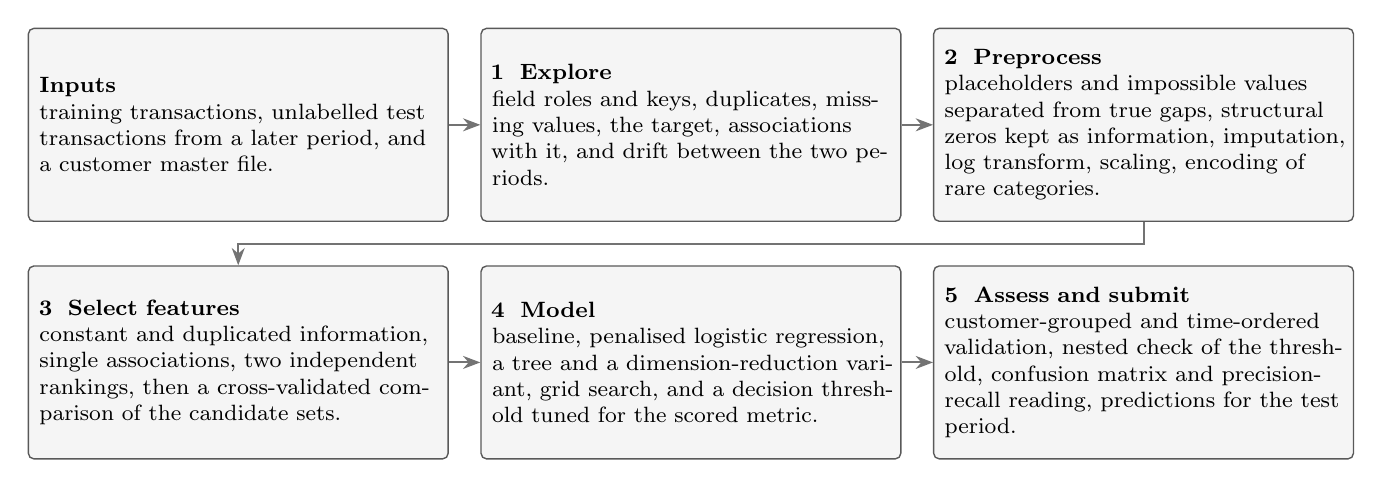
\begin{tikzpicture}[
  font=\footnotesize,
  box/.style={draw=black!65, line width=0.5pt, fill=black!4, rounded corners=2pt,
              text width=5.05cm, minimum height=2.45cm, align=left, inner sep=4pt},
  ar/.style={-{Stealth[length=2.2mm]}, draw=black!55, line width=0.7pt}]

\node[box] (a) {\textbf{Inputs}\\
  training transactions, unlabelled test transactions from a later period, and a customer master file.};

\node[box, right=0.4cm of a] (b) {\textbf{1 \ Explore}\\
  field roles and keys, duplicates, missing values, the target, associations with it, and drift between the two
  periods.};

\node[box, right=0.4cm of b] (c) {\textbf{2 \ Preprocess}\\
  placeholders and impossible values separated from true gaps, structural zeros kept as information, imputation,
  log transform, scaling, encoding of rare categories.};

\node[box, below=0.55cm of a] (d) {\textbf{3 \ Select features}\\
  constant and duplicated information, single associations, two independent rankings, then a cross-validated
  comparison of the candidate sets.};

\node[box, right=0.4cm of d] (e) {\textbf{4 \ Model}\\
  baseline, penalised logistic regression, a tree and a dimension-reduction variant, grid search, and a decision
  threshold tuned for the scored metric.};

\node[box, right=0.4cm of e] (f) {\textbf{5 \ Assess and submit}\\
  customer-grouped and time-ordered validation, nested check of the threshold, confusion matrix and
  precision-recall reading, predictions for the test period.};

\draw[ar] (a) -- (b);
\draw[ar] (b) -- (c);
\draw[ar] (c.south) -- ++(0,-0.28) -| (d.north);
\draw[ar] (d) -- (e);
\draw[ar] (e) -- (f);
\end{tikzpicture}
\end{center}

% ================================================================== 3
\section{The stages and why each one suits this data}

\lead{Preprocessing} A placeholder for an unknown amount is not a large purchase, so those 88 cells and the
impossible negatives became missing values, flagged rather than clipped. An empty purchase history is not missing
at all: 1{,}048 rows belong to customers with no earlier order, so those fields were set to zero and marked.
Amounts are skewed, so a log transform and scaling follow, and rare categories were grouped before encoding.

\lead{Integrating the customer data} The customer file is optional, so it was joined only where it earns its
place, and the key was checked first so no transaction is duplicated. Region and cohort carry real signal: one
region repeats on 94.5\% of its rows, almost 39 points above the average. Street, company name and postal code
were left out: identifiers dressed as features, which would let the model memorise addresses instead of learning
behaviour.

\lead{Feature selection} Selection was made by concept rather than by column, because encoding one category as
several indicators makes those columns dependent. Constant and near-duplicate fields go first, then weak single
associations, then two rankings that disagree in useful ways, and finally a cross-validated comparison that
prefers the smaller set. The funnel runs from 53 concepts and 124 columns to 19 and 64.

\lead{Modelling} With a few thousand rows of tabular, business-readable fields, a penalised logistic regression
is the honest first choice: stable at this size, lightly tuned, and one interpretable coefficient per feature.
A decision tree and a dimension-reduction variant were fitted as checks beside an always-yes baseline; the linear
model won, 0.748 against 0.723 and 0.745.

\lead{Assessment} The same customers appear many times, so a random split tests the model on rows whose customer
already helped fit it; the folds are grouped on the customer. Because the score depends on a decision threshold
as much as on the model, that threshold was tuned on out-of-fold probabilities and re-verified inside a nested
loop. A final check fits the earlier years and scores the later ones.

% ================================================================== 4
\clearpage
\section{Results}

The grouped 0.755 is the honest floor, since those folds use customers the model has never met; the time-ordered
0.795 is the realistic expectation, and the submission's 0.782 sits between them.

\begin{center}
\begin{tabularx}{0.78\textwidth}{@{}R r@{}}
\toprule
\textbf{Measure} & \textbf{F1}\\
\midrule
Always-yes baseline & 0.718\\
Customer-grouped cross-validation & 0.755\\
Time-ordered check, all rows & 0.795\\
\quad returning customers & 0.801\\
\quad first appearance & 0.730\\
Kaggle, public part of the test set & 0.782\\
\bottomrule
\end{tabularx}
\end{center}

\begin{center}
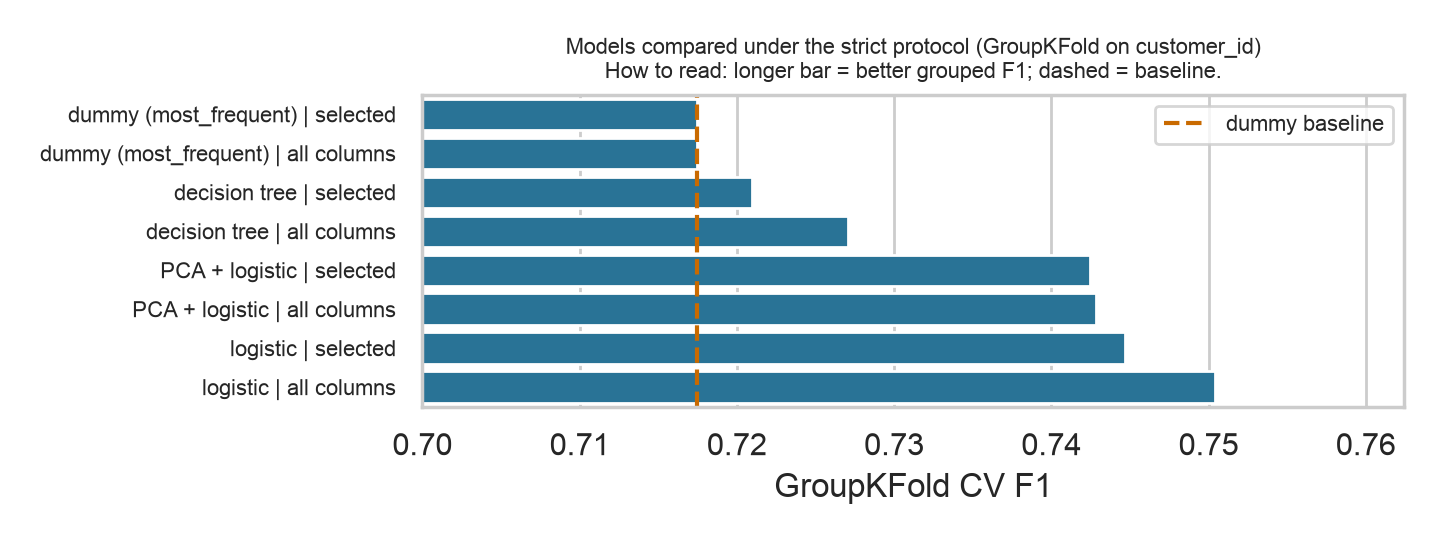
\includegraphics[width=0.61\textwidth]{../artifacts/figures/nb04_model_comparison.png}\\[2pt]
{\small\color{black!60} Figure 1. Every model family under the strict customer-grouped protocol, against the
baseline. The bars sit close together: at this size the honesty of the split matters more than the choice of
algorithm.}\par
\vspace{4pt}
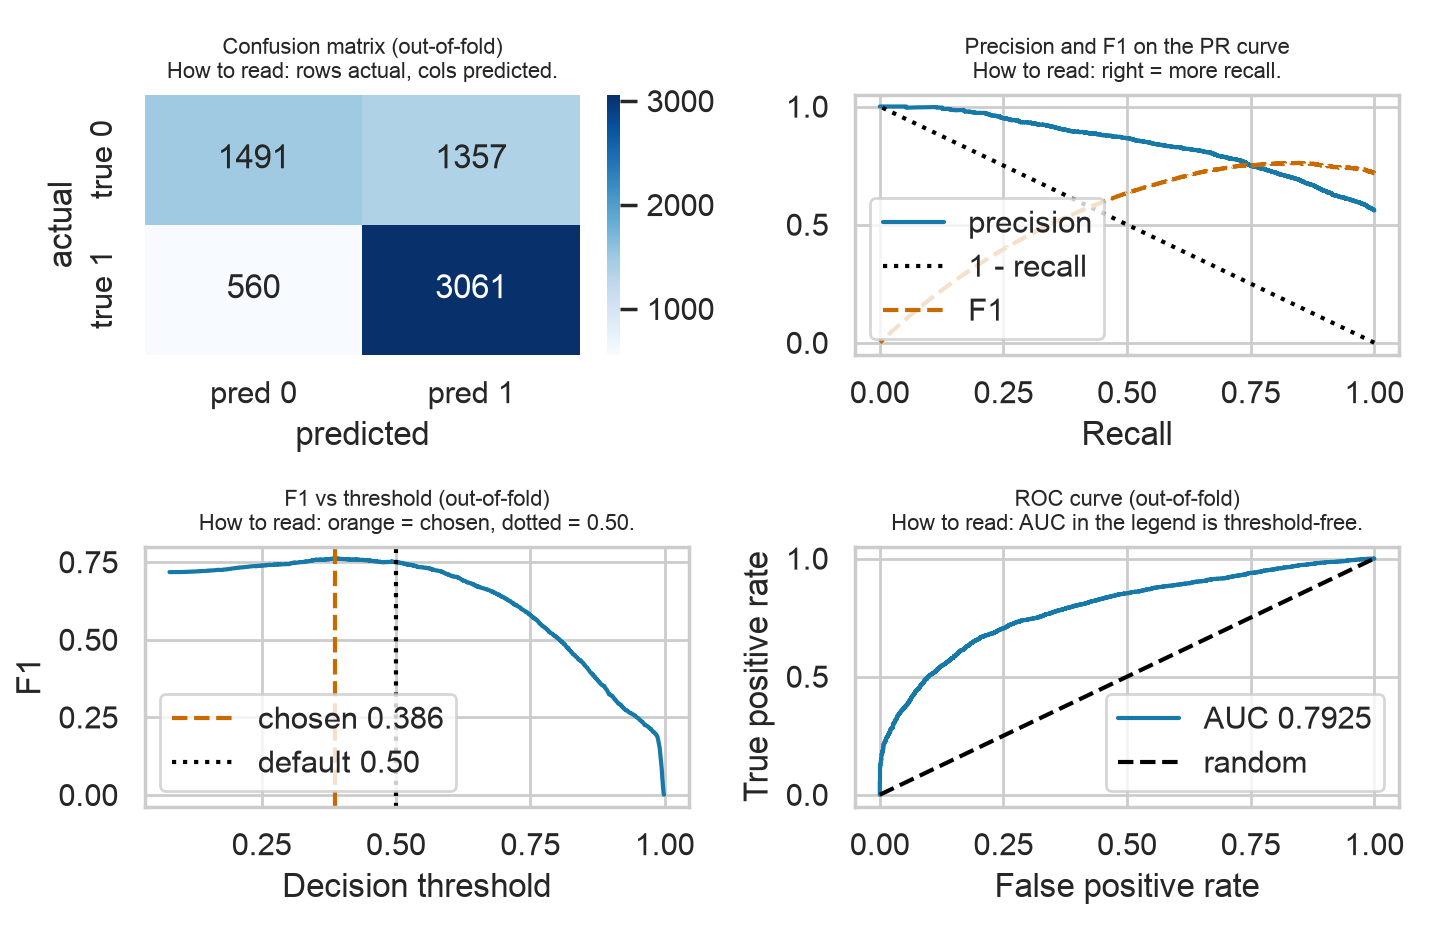
\includegraphics[width=0.61\textwidth]{../artifacts/figures/nb04_assessment.png}\\[2pt]
{\small\color{black!60} Figure 2. The assessment read together: the confusion matrix at the chosen threshold, the
precision-recall trade, the score against the threshold, and the ranking of probabilities on its own.}
\end{center}

% ================================================================== annexes
\section*{\large Annexes}

\anx{A. Reproducing the work} The four notebooks run in sequence in about a minute with a fixed random seed, and
every stage writes its result as a readable table, so any number can be checked afterwards. Only tools covered in
the course were used: no resampling, no bagging, no boosting.

\anx{B. Choices that were tested and then dropped} Customer-level history features, ratios, winsorising, quartile
binning and interactions were all tried; none beat the noise between folds, and the customer aggregates made
things worse. Scaling the yes-no flags as well as the amounts was also worse.

\anx{C. Limitations} The threshold was chosen on the training period and predicts more repeaters than that period
holds, so it is the first value to revisit if the private leaderboard disagrees.

\end{document}
